\documentclass[letter,operight,12pt,spanish]{report}

\usepackage{color}

\usepackage{graphicx}

\usepackage{epsfig}

\usepackage{multirow}

\usepackage{colortbl}

\usepackage[table]{xcolor}

\usepackage{vmargin}

\usepackage[spanish]{babel}

%Gummi|065|=)
\title{\textbf{Robot Cartesiano.}}
\author{Cinematica de Robots.\\
		Ingenieria en Mecatr\'onica 7A}
\date{20 de septiembre de 2019}

\begin{document}

\thispagestyle{empty} %% PARA QUITAR FORMATO DE PIES Y ENCABEZADOS DE PÁGINA A LA PORTADA
%
%
%
%
%
%
%
%   ESPACIO COMENTADO PARA EVITAR DESAJUSTES POR GENERACIÓN DE NUEVO PÁRRAFO (NO DEJAR ESPACIOS ENTRE MINIPAGES)
%
%
%
%
%
%%%%%%%%% MINIPAGE PARA EL LOGO DEL LADO IZQUIERDO (UNIVERSIDAD) %%%%%%%%%%%%%%%%%%%%%%%%%%%%%%%
%
%
%
%
%\fbox{
\begin{minipage}[c][0.15\textheight][c]{0.14\textwidth}
    \begin{center}

\includegraphics[height=2cm, keepaspectratio=true]{/home/sarha13/Escritorio/upzmg.jpeg} %% LOGO IZQUIERDO
    \end{center}
\end{minipage}
%}
%
%
%
%
%
%
%   ESPACIO COMENTADO PARA EVITAR DESAJUSTES POR GENERACIÓN DE NUEVO PÁRRAFO (NO DEJAR ESPACIOS ENTRE MINIPAGES)
%
%
%
%
%
%%%%%%%%%%%%% MINIPAGE PARA EL CUERPO DE LA PORTADA (NOMBRES, TITULOS, ETC.) %%%%%%%%%%%%%%%%%%%%%%%%%%%%%%5
%
%
%
%
%\fbox{
\begin{minipage}[c][0.17\textheight][t]{0.7\textwidth}
    \begin{center}
        {\scshape \Huge Universidad Politecnica ZMG} %% NOMBRE DE LA UNIVERSIDAD
        \vspace{.5cm}   %% DEFINE EL ESPACIO ENTRE EL NOMBRE DE LA UNIVERSIDAD Y LA LÍNEA DOBLE
        \hrule height2.5pt  %% DEFINE EL ANCHO DE LA PRIMER LÍNEA
        \vspace{.1cm}    %% DEFINE EL ESPACIO ENTRE LAS DOS LINEAS
        \hrule height1pt  %% DEFINE EL ANCHO DE LA SEGUNDA LINEA (NORMALMENTE ES MAS DELGADA)
        \vspace{.4cm}   %% DEFINE EL ESPACIO ENTRE LA DOBLE LINEA Y EL NOMBRE DE LA DIVISIÓN
        {\scshape \LARGE Divisi\'on Acad\'emica de Mecatr\'onica}  %% NOMBRE DE LA DIVISIÓN
    \end{center}
\end{minipage}
%}
%
%
%
%
%
%   ESPACIO COMENTADO PARA EVITAR DESAJUSTES POR GENERACIÓN DE NUEVO PÁRRAFO (NO DEJAR ESPACIOS ENTRE MINIPAGES)
%
%
%
%
%
%
%   ESPACIO COMENTADO PARA EVITAR DESAJUSTES POR GENERACIÓN DE NUEVO PÁRRAFO (NO DEJAR ESPACIOS ENTRE MINIPAGES)
%
%
%
%
%
%%%%%%%%%%%%%%%%%%%%%%% MINIPAGE PARA EL LOGO DEL LADO DERECHO (DIVISIÓN ACADÉMICA)
%
%
%
%
%\fbox{
%}
%
%
%
%
%
%    ESPACIO COMENTADO PARA EVITAR DESAJUSTES POR GENERACIÓN DE NUEVO PÁRRAFO (NO DEJAR ESPACIOS ENTRE MINIPAGES)
%
%
%
%
%
%
%%%%%%% RENGLÓN DE ABAJO DEJADO INTENCIONALMENTE EN BLANCO PARA GENERAR NUEVO COMIENZO DE PÁRRAFO  %%%%%%

%%%%%%%%%%%%%%%%%%%%%%%%%%%%%%%%%%%%%%%%%%%%%%%%%%%%%%%%%%%%%%%%%%%%%%%%%%%%%%%%%%%%%%%%%%%%%%%%%%%%%%%%%
%
%
%
%
%
%  ESPACIO COMENTADO PARA EVITAR DESAJUSTES POR GENERACIÓN DE NUEVO PÁRRAFO (NO DEJAR ESPACIOS ENTRE MINIPAGES)
%
%
%
%
%
%
%%%%%%%%%%%%%%%% 5TO MINIPAGE PARA EL CUERPO DE LA PORTADA (NOMBRES, TÍTULO, ETC.) %%%%%%%%%%%%%%%%%%%%%%%%%%%%%%%%%%%%%%
%
%
%
%
%\fbox{
\begin{minipage}[l][0.78\textheight][t]{0.1\textwidth}
    \begin{center}
    \hskip0pt
    \vrule width2.5pt height17cm    %% height definde la altura de la linea gruesa
        \hskip1mm
        \vrule width1pt height17cm  %% height define la altura de la linea delgada
        \end{center}
\end{minipage}
%}
%\fbox{
\begin{minipage}[c][0.78\textheight][t]{0.8\textwidth}
      \begin{center}
      \vspace{2cm}
        {\Large \scshape {Robot Catersiano}}

        \vspace{2cm}

        \makebox[5cm][c]{\LARGE Proyecto}  \\[20pt]
        Que para obtener el t\'itulo de:\\[5pt]
        {\Large \textbf{{Ingeniero en Mecatronica}}}\\[40pt]
        PRESENTA:\\[12pt]
        \textbf{ \Large {Alcala Villagom\'e Mario.\\
        				Becerra I\~niguez Diego Armando.\\
        				Martinez Velazquez Lisbeth.\\
        				Murgu\'ia Ch\'avez Nadia Sarahi.\\
        				Ramos Ch\'avez Brayan Oswaldo.}}

        \vspace{2cm}

        { \small Directores}:\\ {Ing. Moran Grabito Carlos Enrique}\\{Ing. Razo Cerda Rosa Mar\'ia}
        \vspace{2.5cm}

        { Tlajomulco de Zuñiga, Jalisco} \hskip2.5cm {Septiembre de 2019}
      \end{center}
\end{minipage}
%}

\maketitle

\section{Problematica}

Dentro las farmaceuticas con alta demanda como los el IMSS (Instituto M\'exicano del Seguro Social) y algunas otras de dependencia privada se presenta el almacenamiento de medicamentos, as\'i como una atenci\'on al cliente lenta y deficiente, ya que el sutimiento de recetas medicas resulta algo tardado y de tiempo, pues no se tiene un orden correcto.
\subsection{Objetivo General}

Elaboraci\'on de un robot cartesiano para la implementaci\'on dentro del \'area de sutimiento de medicamentos\\

\subsubsection{Objetivos del proyecto}

$\diamond$ Modelaci\'on matematica de un sistema robotizado.

$\diamond$ Diseño y simulaci\'on de mecanismos.

$\diamond$ Administraci\'on y control de recursos economicos y humanos.

$\diamond$ Selecci\'on y elecci\'on de sensores y actuadores.

\subsection{Justificaci\'on}

La implementaci\'on de del robot cartesiano dentro del \'area farmaceutica sea visto de manera concreta ya que la labor a desempeñar de este seria el surtimiento de medicamentos y el mejoramiento de la atenci\'on al cliente

Buscando mejorar la atencion al cliente al momento de ir a surtir sus medicamentos y un mejor desempeño laboral para los farmaceuticos que pierdes horas en buscar los medicamntos en los almacenes.

\subsection{Delimitaci\'on}

Dentro de la implementaci\'on del robot en una \'area donde el lugar el reducido, as\'i como su implentacion dentro de un \'area publica se debe contar con los requisistos y estandares de seguridad que marca el IMSS. Al igual que debe ser facil de operar.
\section{Cronograma de actividades}

\subsection{Matriz de posibles materiales y costos}

\begin{center}
\begin{tabular}{|l|c|}
\hline
	\textbf{Materiales} & \textbf{costo}\\
\hline
	Servo motores & 5,000\\
\hline
	Drivers & 4,500\\
\hline
	Aluminio & 7,000\\
\hline
	Cables & 200\\
\hline
	Motor de cremallera & 1,000\\
\hline
	Total & 17,700\\
\hline
\end{tabular}
\end{center}

\subsection{Matriz de roles}

\begin{center}
\begin{tabular}{|c|l|}
\hline
	\textbf{Signo} & \textbf{Leyenda}\\
\hline
	P & Responsabilidad\\
\hline
	C & Colabora\\
\hline
	I & Suministra informaci\'on a los dem\'as\\
\hline
	MN & Mario Alcala Villagom\'ez y Nadia Sarahi Murgu\'ia Ch\'avez\\
\hline
	DB & Diego Armando Becerra Iñiguez y Brayan Oswaldo Ramos Ch\'avez\\
\hline
	LN & Lisbeth Martinez Velazquez y Nadia Sarahi Murgu\'ia Ch\'avez\\
\hline
\end{tabular}
\end{center}

\subsection{Diagrama Gantt}

\begin{center}
\begin{tabular}{|l|c|c|c|c|}
\hline
	\textbf{Actividades} & \textbf{MN} & \textbf{DB} & \textbf{LN} & \textbf{Fecha}\\
\hline
	Titulo del proyecto & P & C & I & 16 al 20 septiembre\\
\hline
	Planteamiento del problema & I & P & C & 16 al 20 septiembre\\
\hline
	Formular el Problema & I & C & P & 16 al 20 septiembre\\
\hline
	Objetivo general del proyecto & P & I & C & 16 al 20 septiembre\\
\hline
	Objetivos del proyecto & P & C & I & 16 al 20 septiembre\\
\hline
	Justificaci\'on & C & C & P & 16 al 20 septiembre\\
\hline
	Delimitaci\'on & C & I & P & 16 al 20 septiembre\\
\hline
	Matriz de posibles costos materiales & P & C & I & 16 al 20 septiembre\\
\hline
	Matriz de roles & I & C & P & 16 al 20 septiembre\\
\hline
	Diagrama de Gantt & P & I & C & 16 al 20 septiembre\\
\hline
	Explicaci\'on de la aportaci\'on de cada materia & C & P & I & 16 al 20 septiembre\\
\hline
	Desarroyollo del proyecto & P & C & IP & -\\
\hline
	Bibliograf\'ia & PI & CI & IP & -\\
\hline
	Total P & 7 & 2 & 6 & -\\
\hline
	Total C & 3 & 8 & 3 & -\\
\hline
	Total I & 4 & 4 & 6 & -\\
\hline
\end{tabular}
\end{center}

\newpage

\section{Relaci\'on de materias}

\begin{center}
\begin{tabular}{|l|l|}
\hline
	\textbf{Materias de 7to} & \textbf{Detalles de la Aportanci\'on al proyecto}\\
\hline
	\textbf{Ingles VII} & Comprenci\'on y Ttraduccion de articulos, libros\\
	& y manuales consultados.\\
\hline
	\textbf{Termodinamica} & Analisis de temperatura en el sistema robotico\\
\hline	
	\textbf{Modelado de sistemas} & Modelado matematico para el an\'alisis\\
	& cinematico del robot, mediante calculos\\
\hline
	\textbf{Administraci\'on y de proyectos} & Gesti\'on y organizacion, planeaciones\\
	& y control de recursos economicos, materiales\\
	& y humanos.\\
\hline
	\textbf{Cinematica de robots} & Calculo y especificaciones matematicas\\
	& para la correcta estuturaci\'on del robot\\
\hline
\textbf{Dise\~no} & Dise\~no y simulaci\'on de la estructura del robot\\
\hline
\end{tabular}
\end{center}

\newpage

\section{Diseño CAD del robot}

Para el diseño CAD se realizo el siguiente bocea a papel, dando una \'idea general de como estaria el robot.(ver la Fig. 1), el cual se trata de posicionar en laa estanteria de los medicamentos para que este los tome y elos lleve a un deposito donde el farmaceutico pueda tomarlos facilmente.\\

\begin{figure}[htp]
\centering
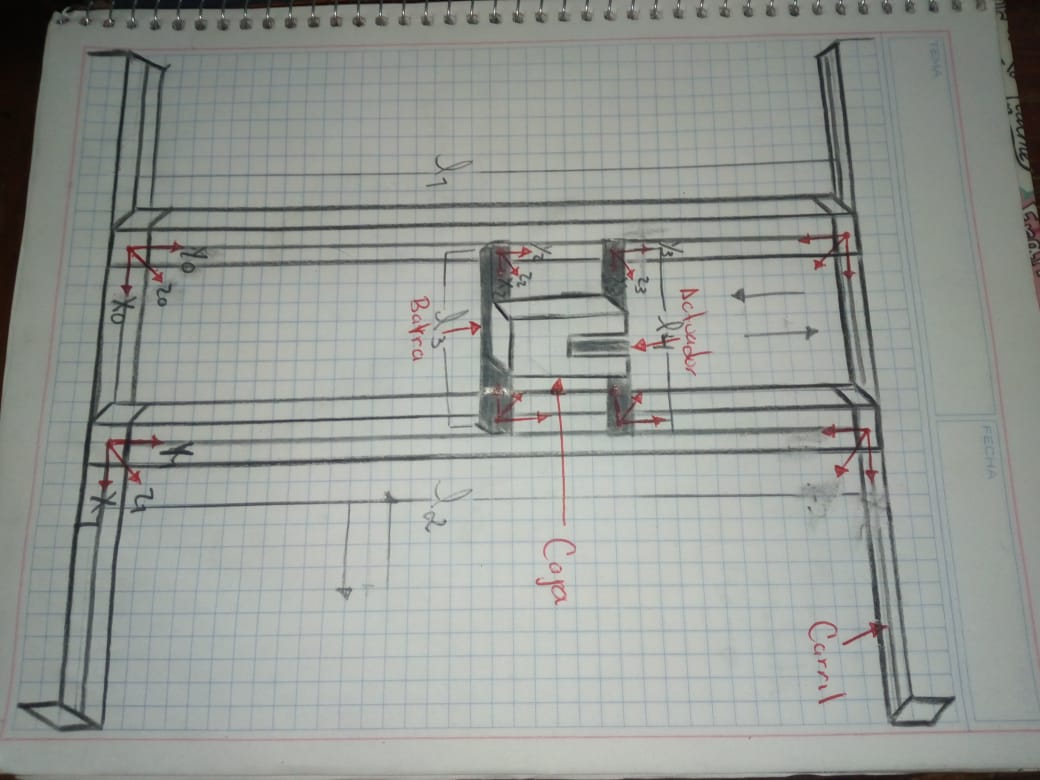
\includegraphics[width=8cm]{/home/sarha13/Escritorio/Boceto.jpeg}
\caption{Boceto}
\label{Fig. 1}
\end{figure}

Realizando las siguentes figuras en el cada empesando por los rieles verticales (50 cm)y horizontales (30 cm).(ver Fig. 2 y Fig. 3)Las cuales haran un movimiento de izquierda a derecha para el dezplazamiento del robot, usando dos barras (30 cm) posicionados en techo y pared para que el robot se pueda mover facilmente por la estanteria.\\\\

\begin{figure}[htp]
\centering
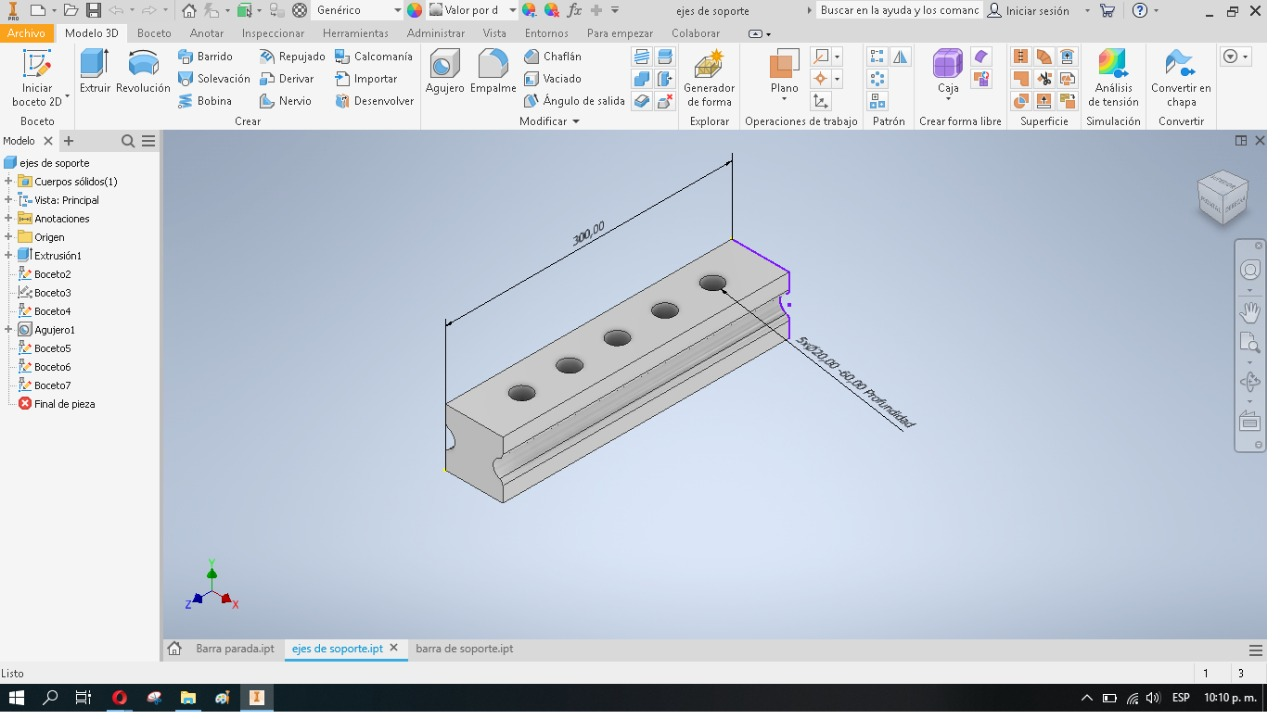
\includegraphics[width=8cm]{/home/sarha13/Escritorio/barravertical.jpeg}
\caption{Barra Vertical}
\label{Fig. 2}
\end{figure}

\begin{figure}[htp]
\centering
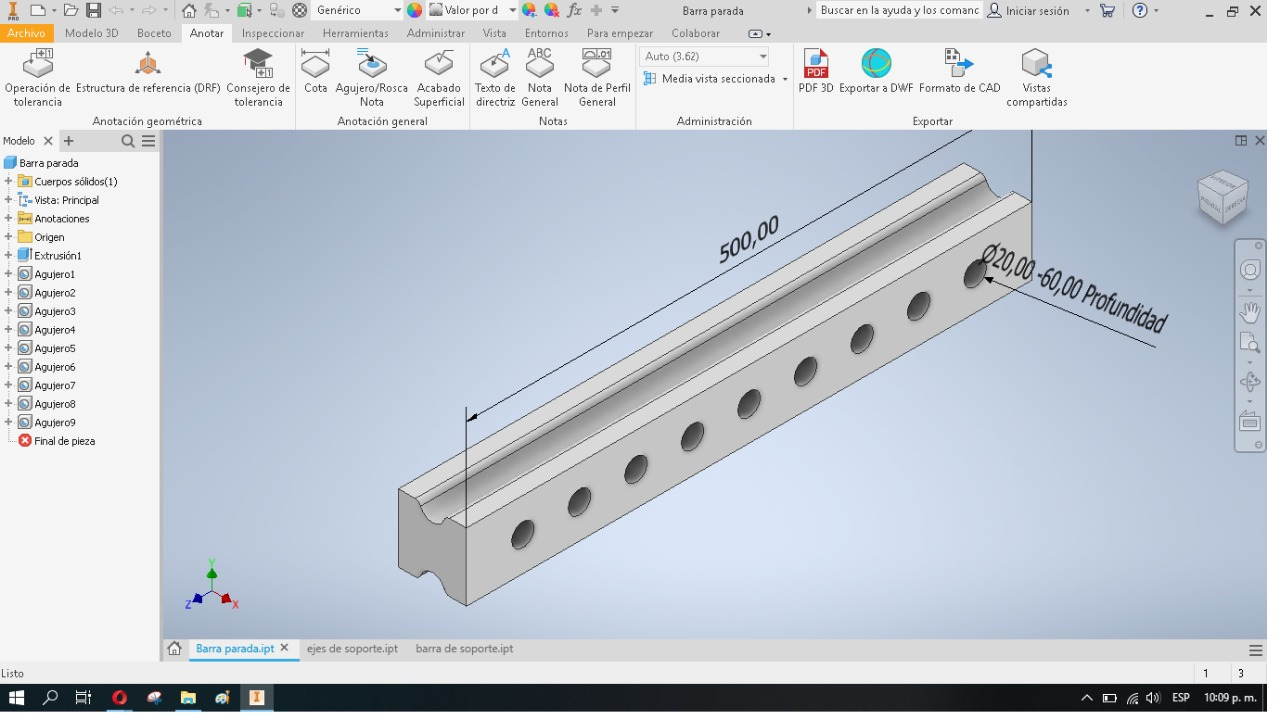
\includegraphics[width=8cm]{/home/sarha13/Escritorio/barrahorizontal.jpeg}
\caption{Barra Horizontal}
\label{Fig. 3}
\end{figure}

Y se utilizara un motor neva para el movimiento del robot.(ver Fig. 4)\\

\begin{figure}[htp]
\centering
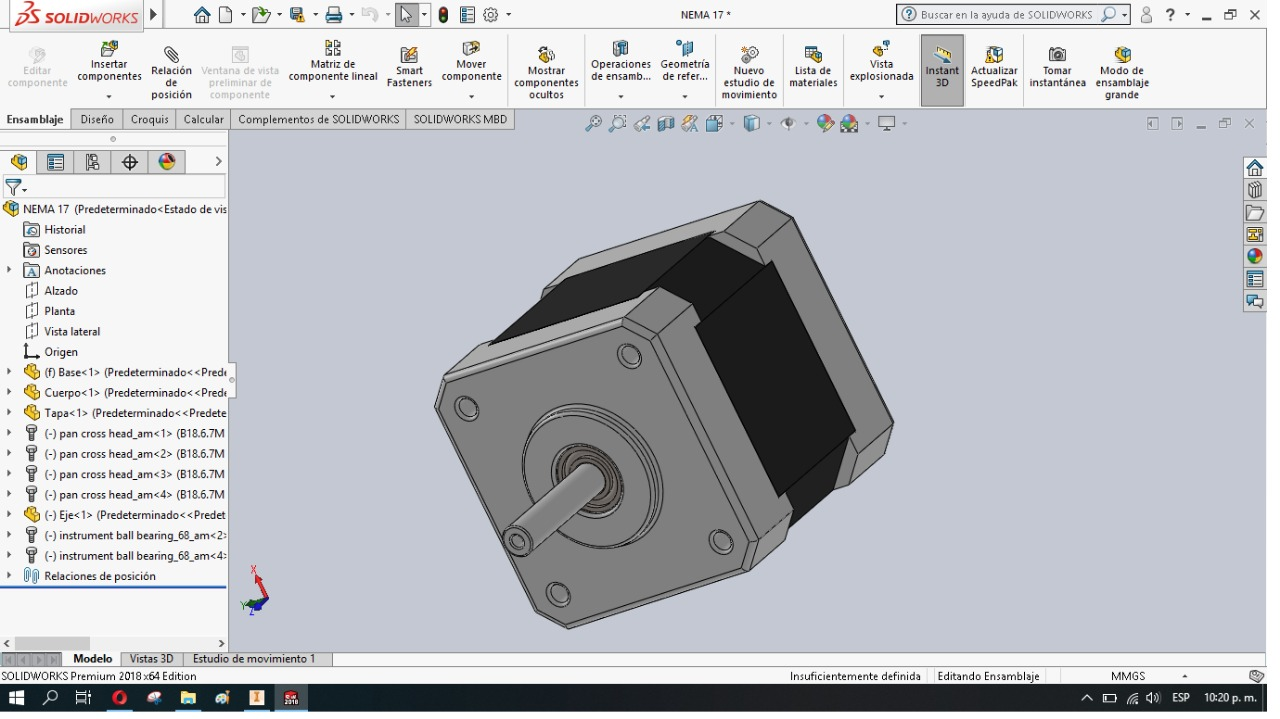
\includegraphics[width=8cm]{/home/sarha13/Escritorio/motorneva.jpeg}
\caption{Motor Neva}
\label{Fig. 4}
\end{figure}

\section{Movilidad}

DISMEDIC tienen una secuencia de movimientos de acuerdo a las coordenadas establecidas para el abastecimiento de medicamentos dentro de las farmacias. Con el cual se busca reducir el tiempo y el mejoramiento de la atenci\'on al cliente al momento de de surtir su receta.\\
La secuencia de movimientos consta de movimientos verticales y horizontales dentro del eje $"x"$ e $"y"$.\\
Es decir que las barras paralelas se mueven de izquierda a derecha y viceversa de manera paralela para posicionarse en el espacio solicitado donde se encuentra el medicamento.\\
En la parte del actuador o surtidor de medicamentos cuenta con dos barras horizontales las cuales se moveran de arriba a bajo y viceverza para tomar tomar el medicamento.\\

\begin{center}
\begin{tabular}{|c|c|c|c|c|}
\hline
	Eje & $\theta_i$ & $d_{i-1}$ & $\alpha_{i-1}$ & $a_i$\\
\hline
	1 & $\theta$ & $\theta$ & $\theta$ & $l_1$\\
\hline
	2 & $\theta$ & $\theta$ & $\theta$ & $l_2$\\
\hline
	3 & $\theta$ & $d_5$ & $\theta$ & $l_3$\\
\hline
	4 & $\theta$ & $d_6$ & $\theta$ & $l_4$\\
\hline
\end{tabular}
\end{center}

\end{document}
